\documentclass[aspectratio=169]{beamer}
\usepackage{xcolor}
\usepackage{multicol}
\usepackage{hyperref}
\usepackage{amsmath}
\usepackage{physics}
\usepackage{setspace}

\usepackage[style=science,backend=biber]{biblatex}
\addbibresource{presentation.bib}

% Metadata of the presentation
\title{Explaining graph neural networks for chemical applications with structure aware games}
\subtitle{}
\author[DB]{Xander Wieme --- \texttt{xander.wieme@ugent.be}}
\date{}

% Macro aimed at loading themes in different directories
\makeatletter
  \def\beamer@calltheme#1#2#3{%
    \def\beamer@themelist{#2}
    \@for\beamer@themename:=\beamer@themelist\do
    {\usepackage[{#1}]{\beamer@themelocation/#3\beamer@themename}}}

  \def\usefolder#1{
    \def\beamer@themelocation{#1}
  }
  \def\beamer@themelocation{}

% Load the UGent theme
\usefolder{theme}
\usetheme[language=en,faculty=we,usecolors]{ugent}
\useinnertheme{ugent}
\useoutertheme{ugent}
\usecolortheme{ugent}
\usefonttheme{ugent}

% Path to images
\graphicspath{{theme/}}

% Have this if you'd like section slides 
\AtBeginSection[]{
    \sectionframe
}

\usepackage{booktabs}

%Images used in the presentation should be stored in the img folder

\begin{document}

\setstretch{1.5}

% Have this if you'd like the presentation to start 
% with a large UGent logo
\logoframe

% I guess you always want a titleframe
\titleframe

% Have this if you'd like a frame containing the 
% table of content
% \begin{frame}{Overview}
%     \tableofcontents[hideallsubsections]
% \end{frame}

\setstretch{1}

\begin{frame}{Molecular property prediction using machine learning}

    \begin{figure}[h]
        \centering 
        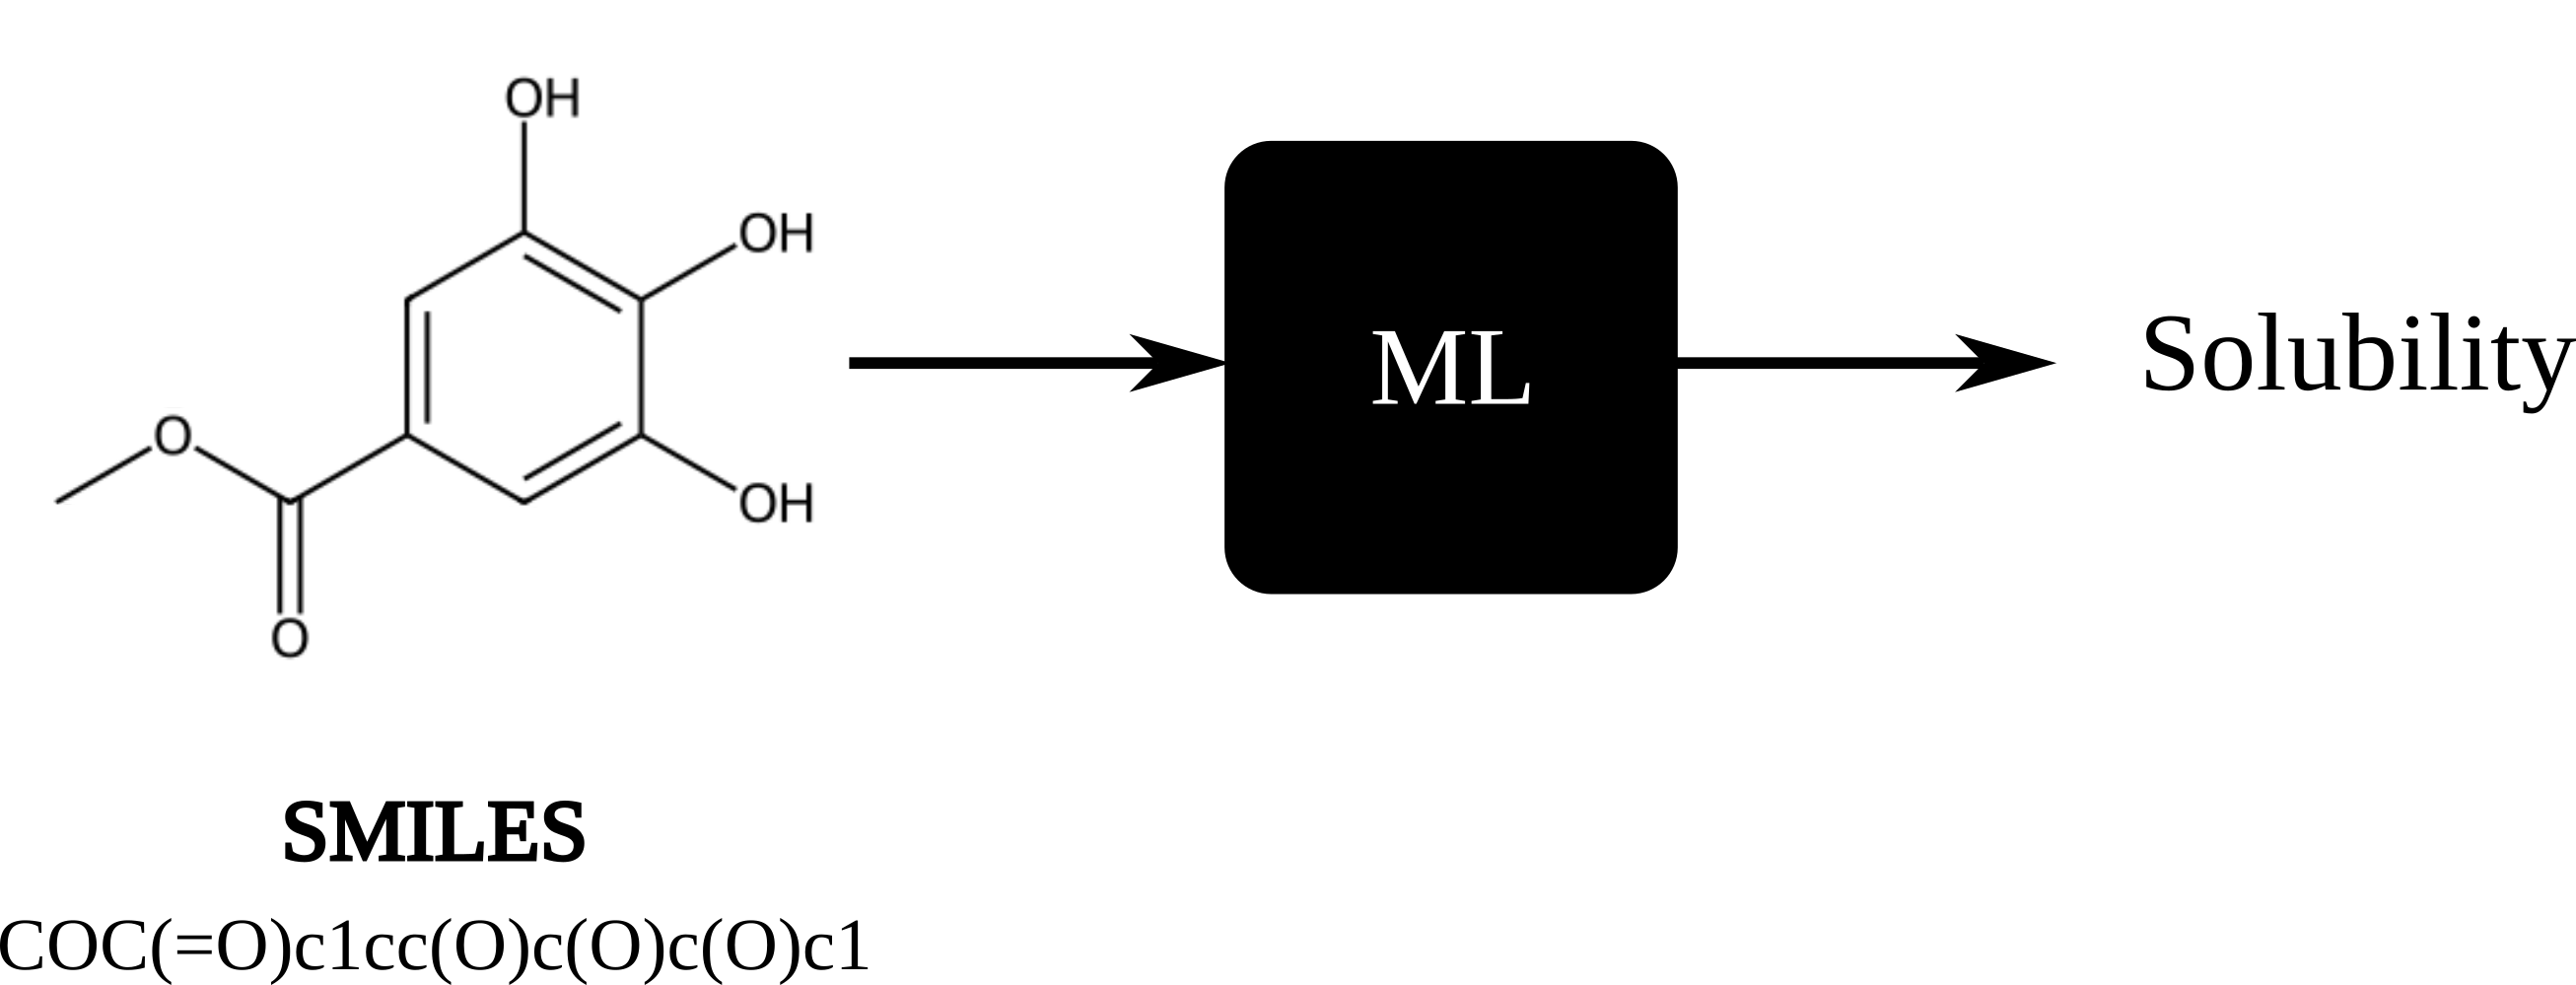
\includegraphics[scale=0.85]{./img/mpp.png}
    \end{figure}
   
\end{frame}


\begin{frame}{XAI: Substructure Mask Exploration (SME)}

    \begin{figure}[h]
        \centering 
        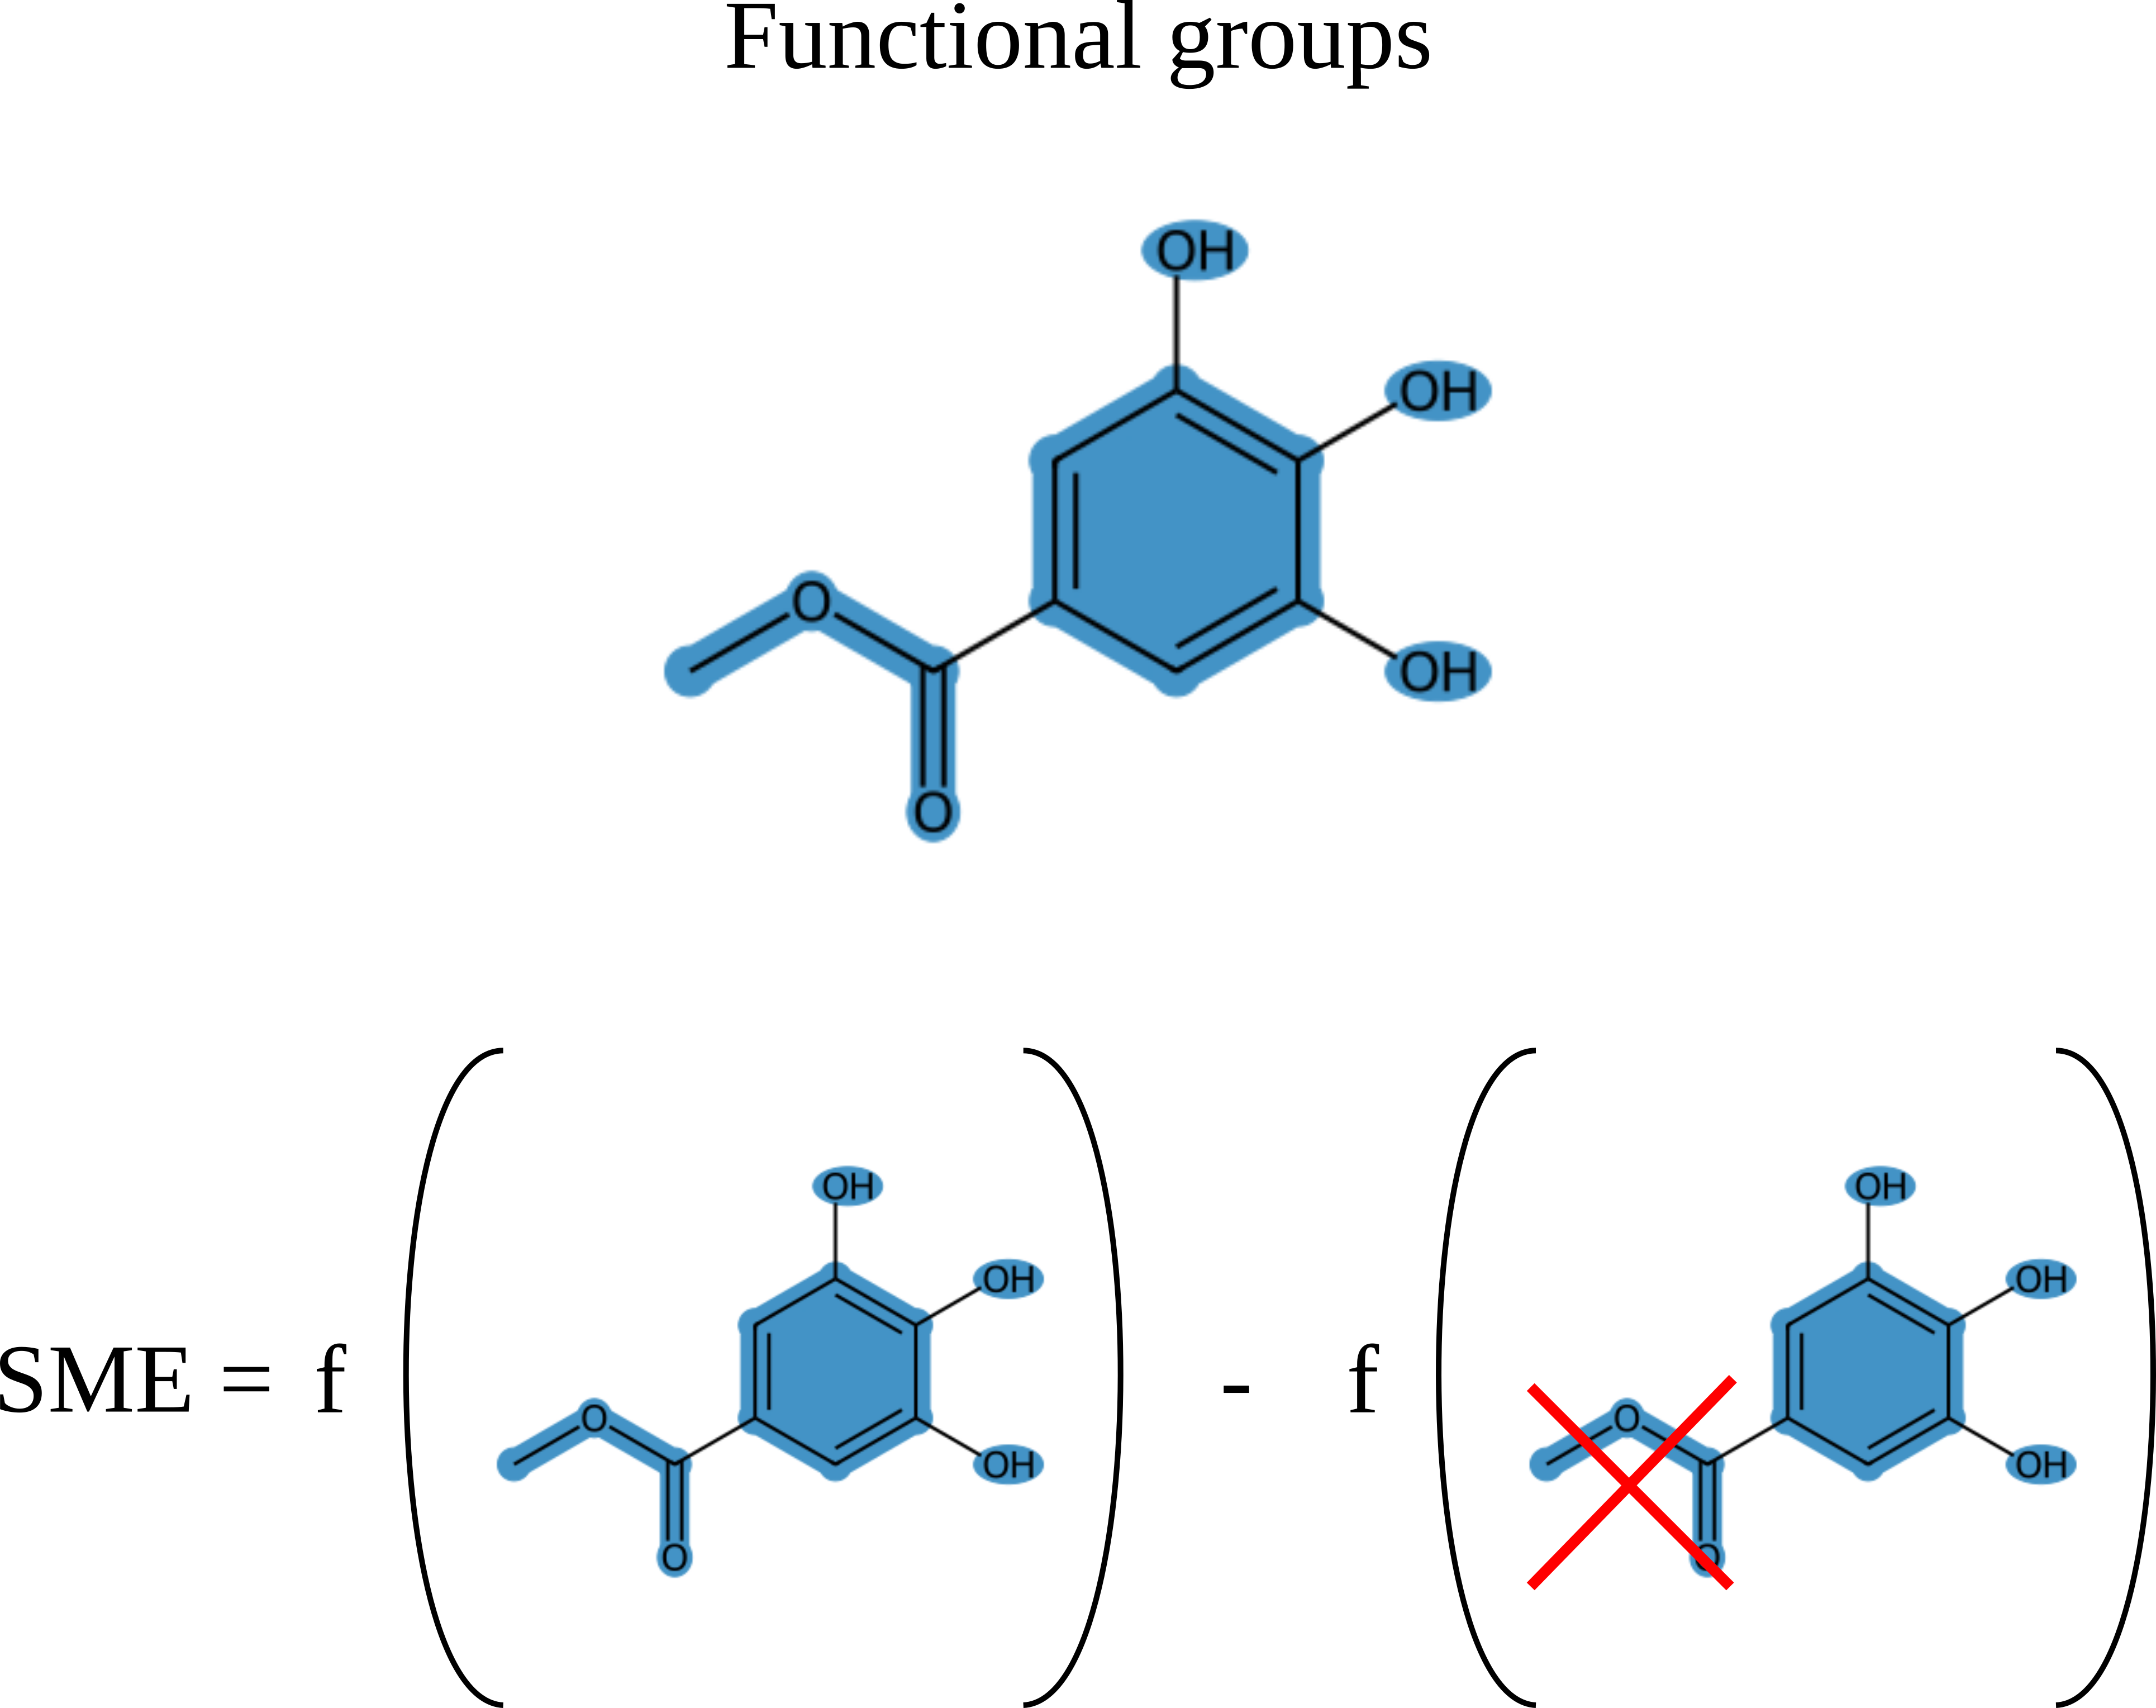
\includegraphics[scale=0.40]{./img/SME.png}
    \end{figure}
    
\end{frame}


\begin{frame}{XAI: Shapley value\footnote[frame]{\fullcite{merrick2020explanation}}}


    \begin{itemize}[<+->]
        \item A cooperative game with transferable utility is
        a pair $(N, v)$ consisting of a set of players $N$ 
        and a characteristic function $v(S) = f(S) - \mathbb{E}[f(G)]$.

        \item Marginal contribution \begin{equation}
            m(i, S) = v\left(S \cup \{i\}\right) - v\left(S\right), \; \text{with } S \subseteq N \setminus \{i\}.
        \end{equation}

        \item Shapley value \begin{center}
            \begin{align}
                \phi_i &= \underset{\pi}{\mathbb{E}} \left[ m\left(i, S_{\pi, i} \right) \right] \\
                    &= \sum_{S \subseteq N \setminus \{i\}} \frac{\left(|N| - 1 - |S|\right)!|S|!}{|N|!} m(i, S)
            \end{align}
        \end{center}
    \end{itemize}
       
\end{frame}


\begin{frame}{XAI: Hamiache-Navarro (HN) value}

        \begin{figure}[h]
            \centering
            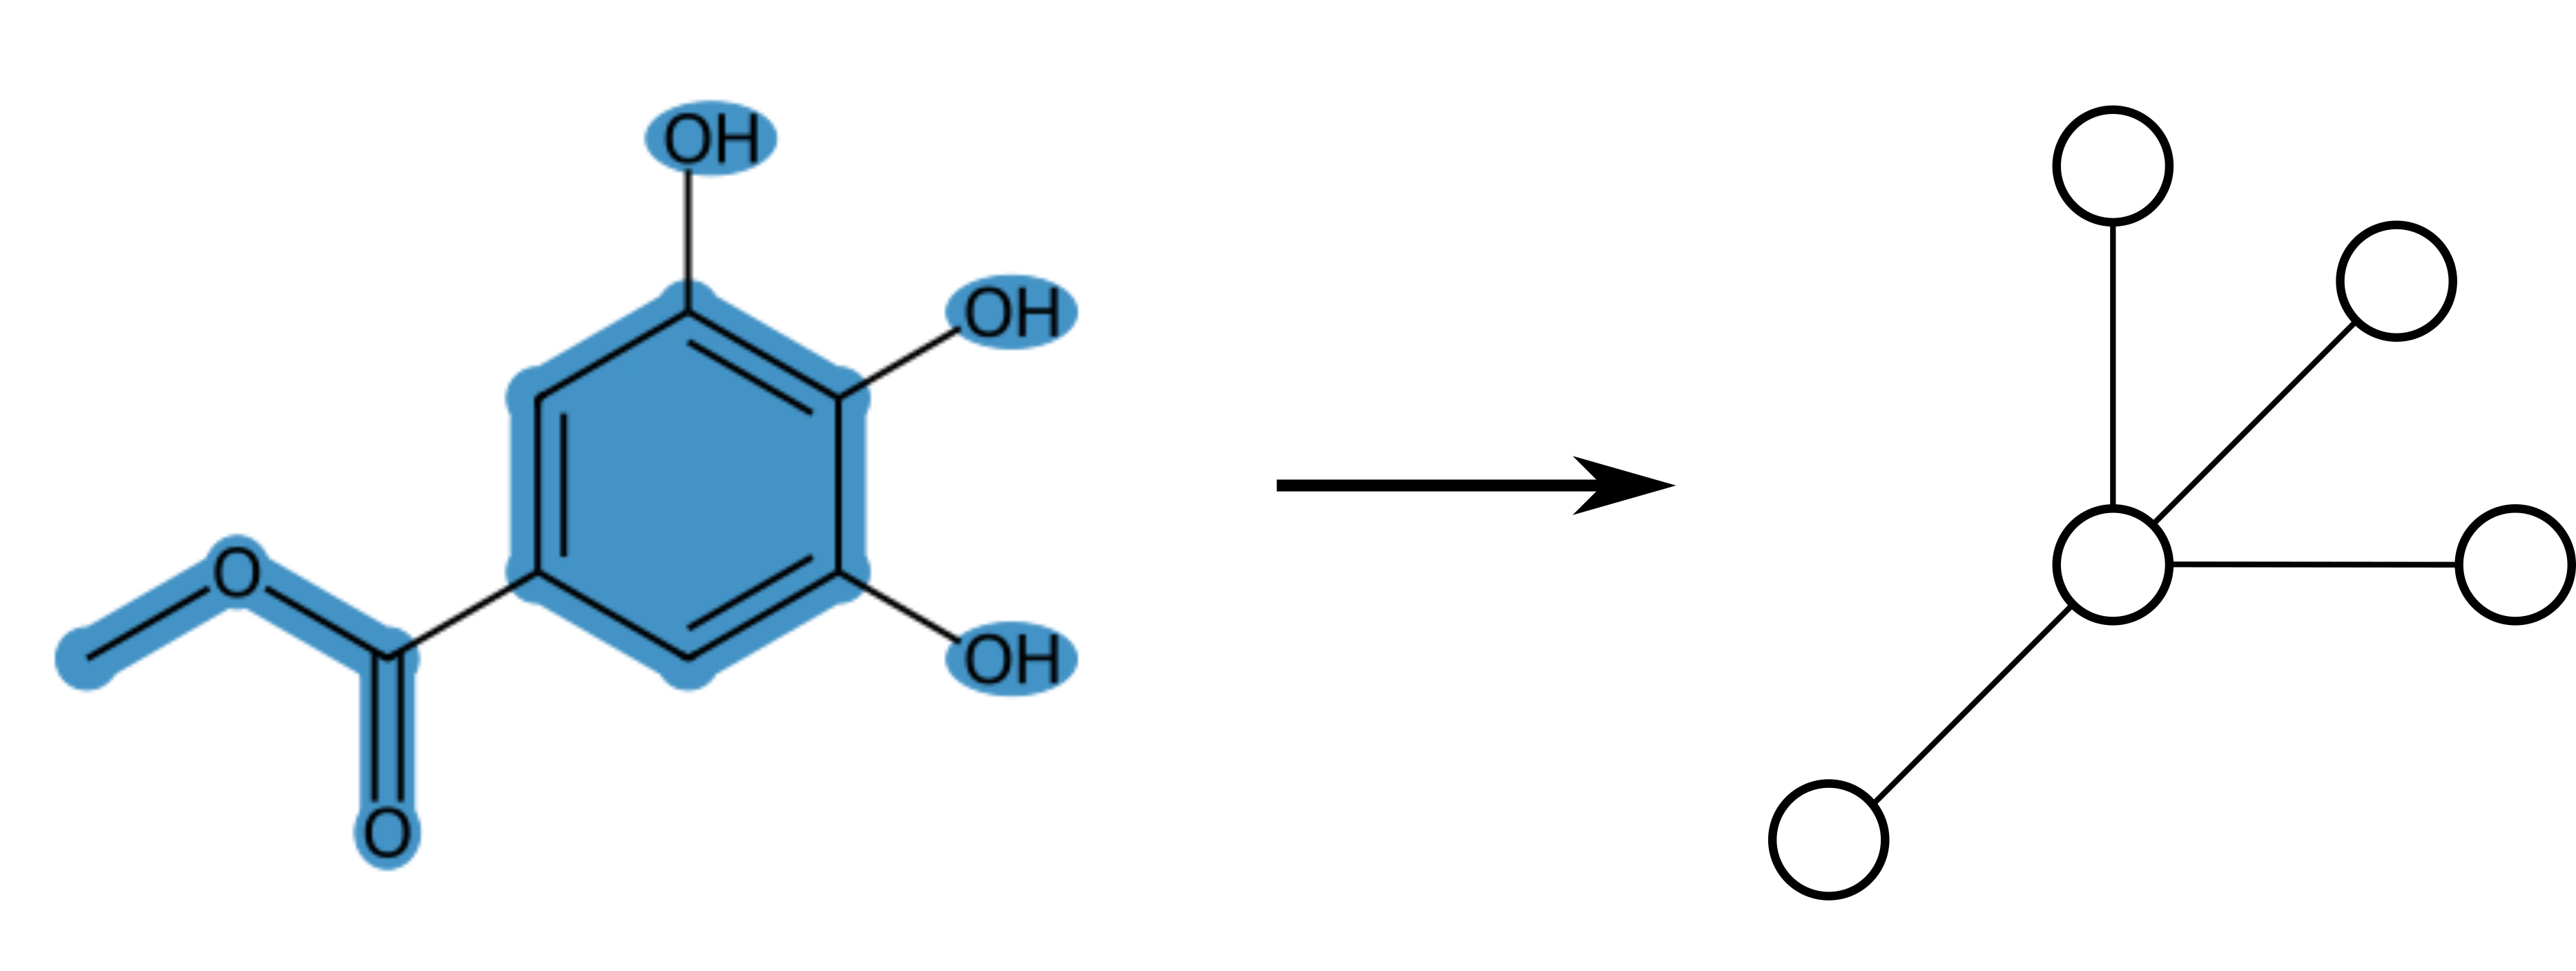
\includegraphics[scale=0.6]{./img/why_HN_value.png}
        \end{figure}

\end{frame}

 
\begin{frame}{Message Passing Neural Networks (MPNN)}

    \begin{figure}[h]
        \centering 
        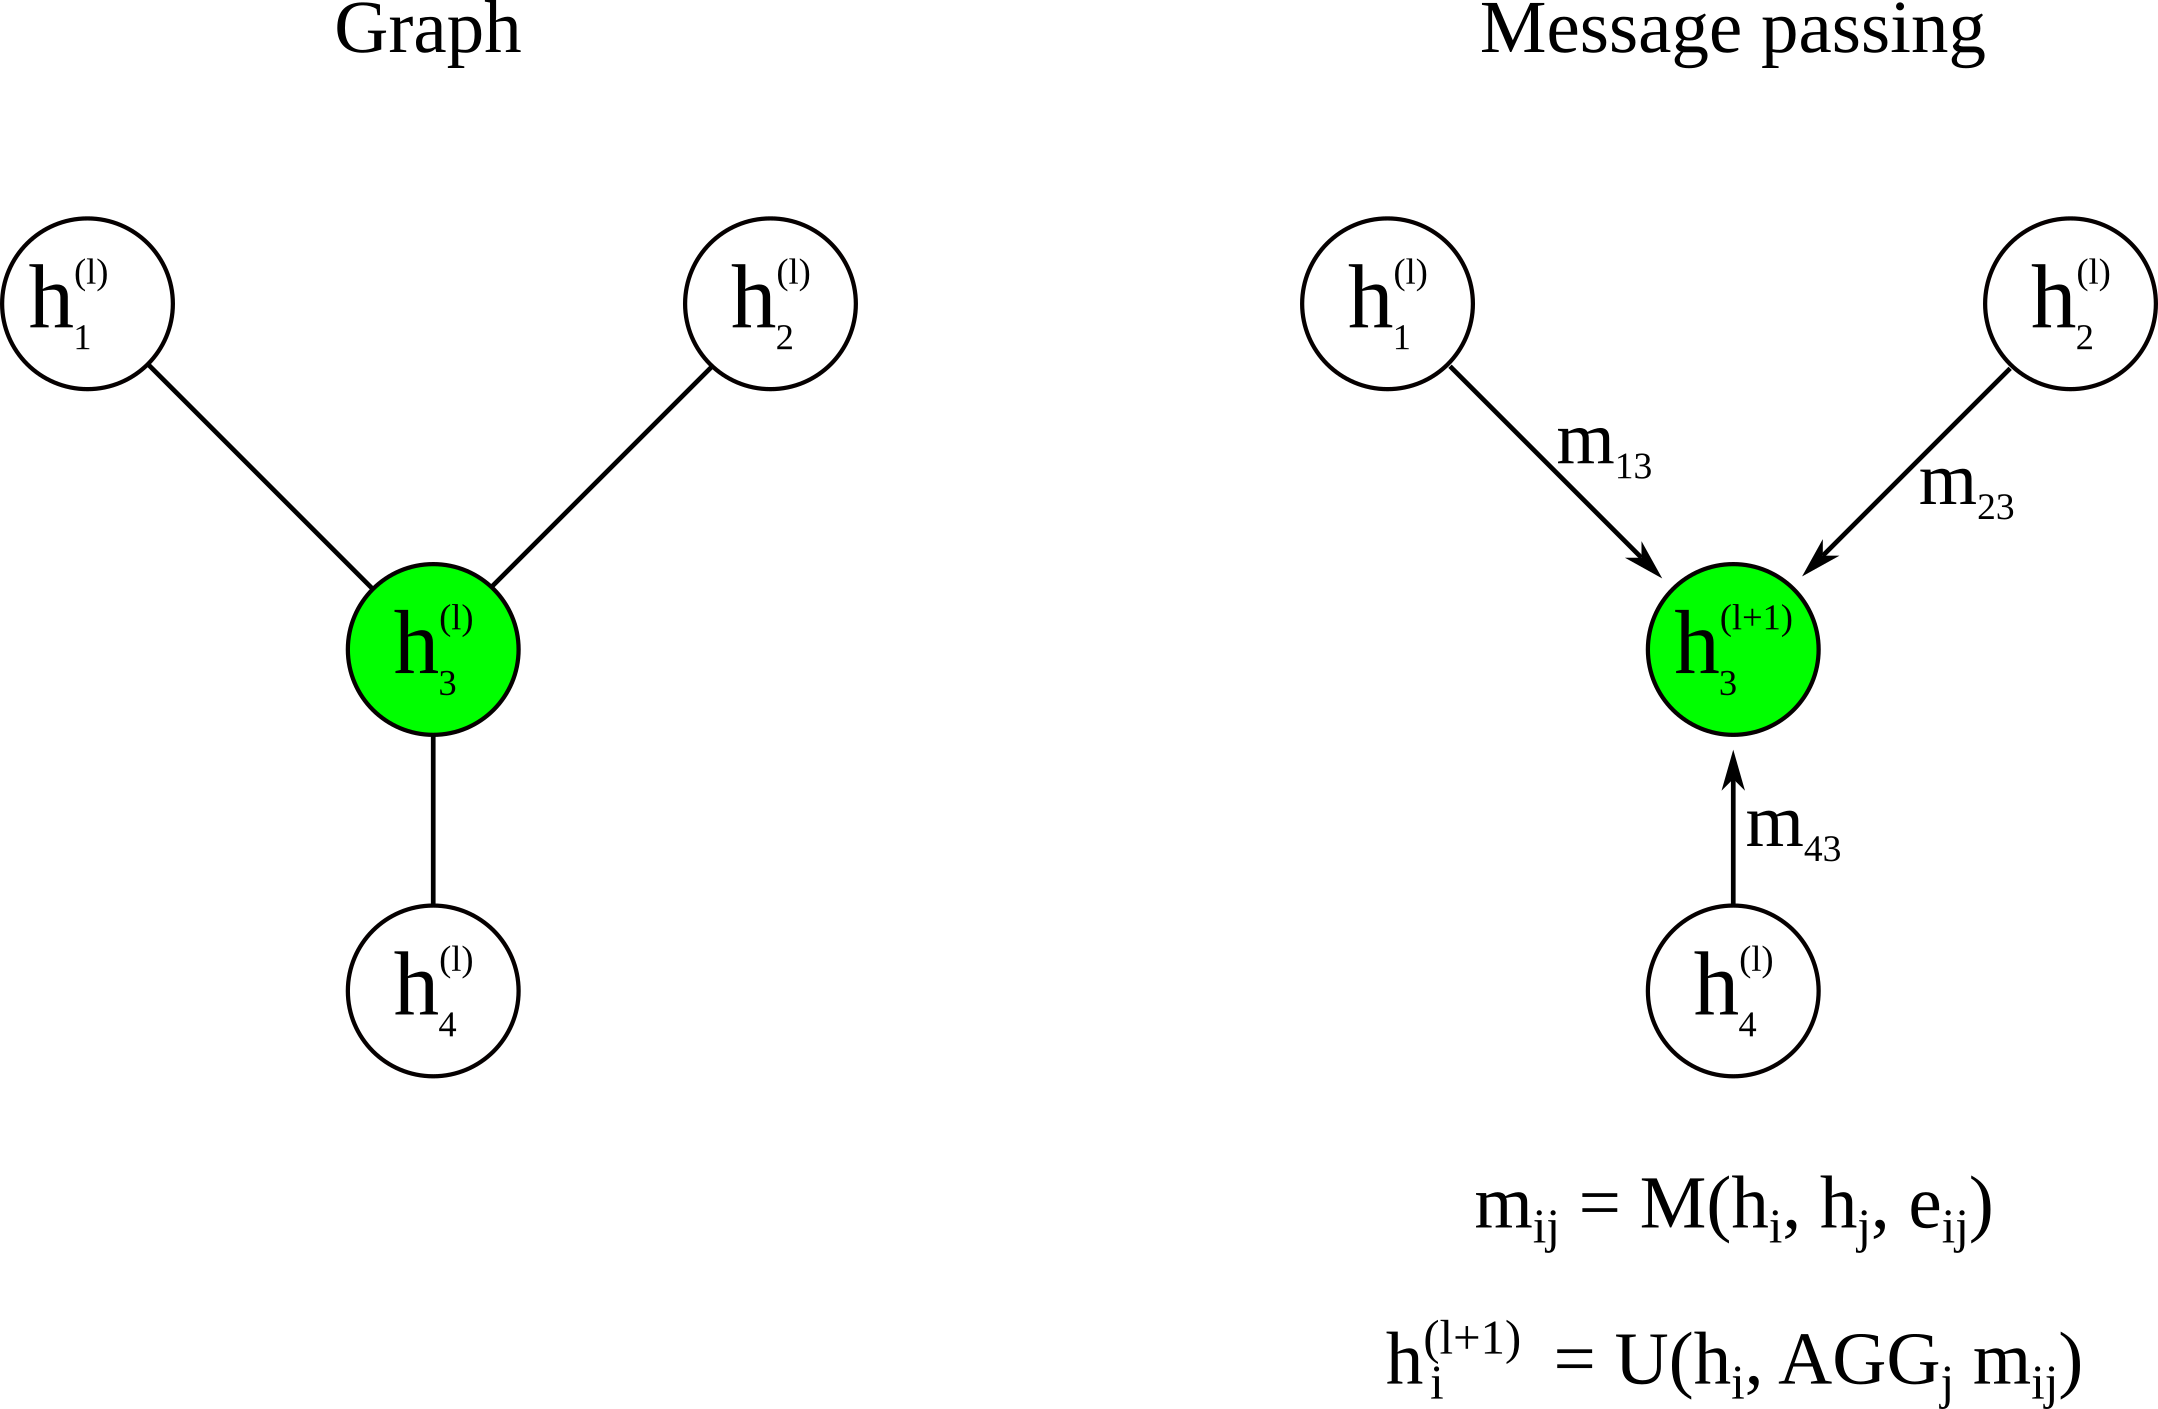
\includegraphics[scale=0.85]{./img/mpnn.png}
    \end{figure}

\end{frame}


\begin{frame}{XAI: Hamiache-Navarro (HN) value}

    \begin{itemize}[<+->]
        \item A cooperative game with incomplete communication is a tuple 
        $(N, v, g)$, where the communication structure is given by 
        the graph $g$.

        \item Associated game using message passing 
            \begin{equation}
                \label{eq:associated_game}
                v^*(S) =
                \begin{cases}
                    \displaystyle
                    v(S) + \tau \sum_{j \in \mathcal{N}(S)} \left[ v(S \cup \{j\}) - v(S) - v(\{j\}) \right] & \text{if } |S/g| = 1 \\
                    \displaystyle
                    \sum_{R \in S/g} v^*(R)                                                                   & \text{otherwise}
                \end{cases}
            \end{equation}

        \item HN value $\phi_i = \tilde{v}(i)$
    \end{itemize}

\end{frame}


\begin{frame}{Relational Graph Neural Networks (RGNN)}

    \begin{figure}[h]
        \centering
        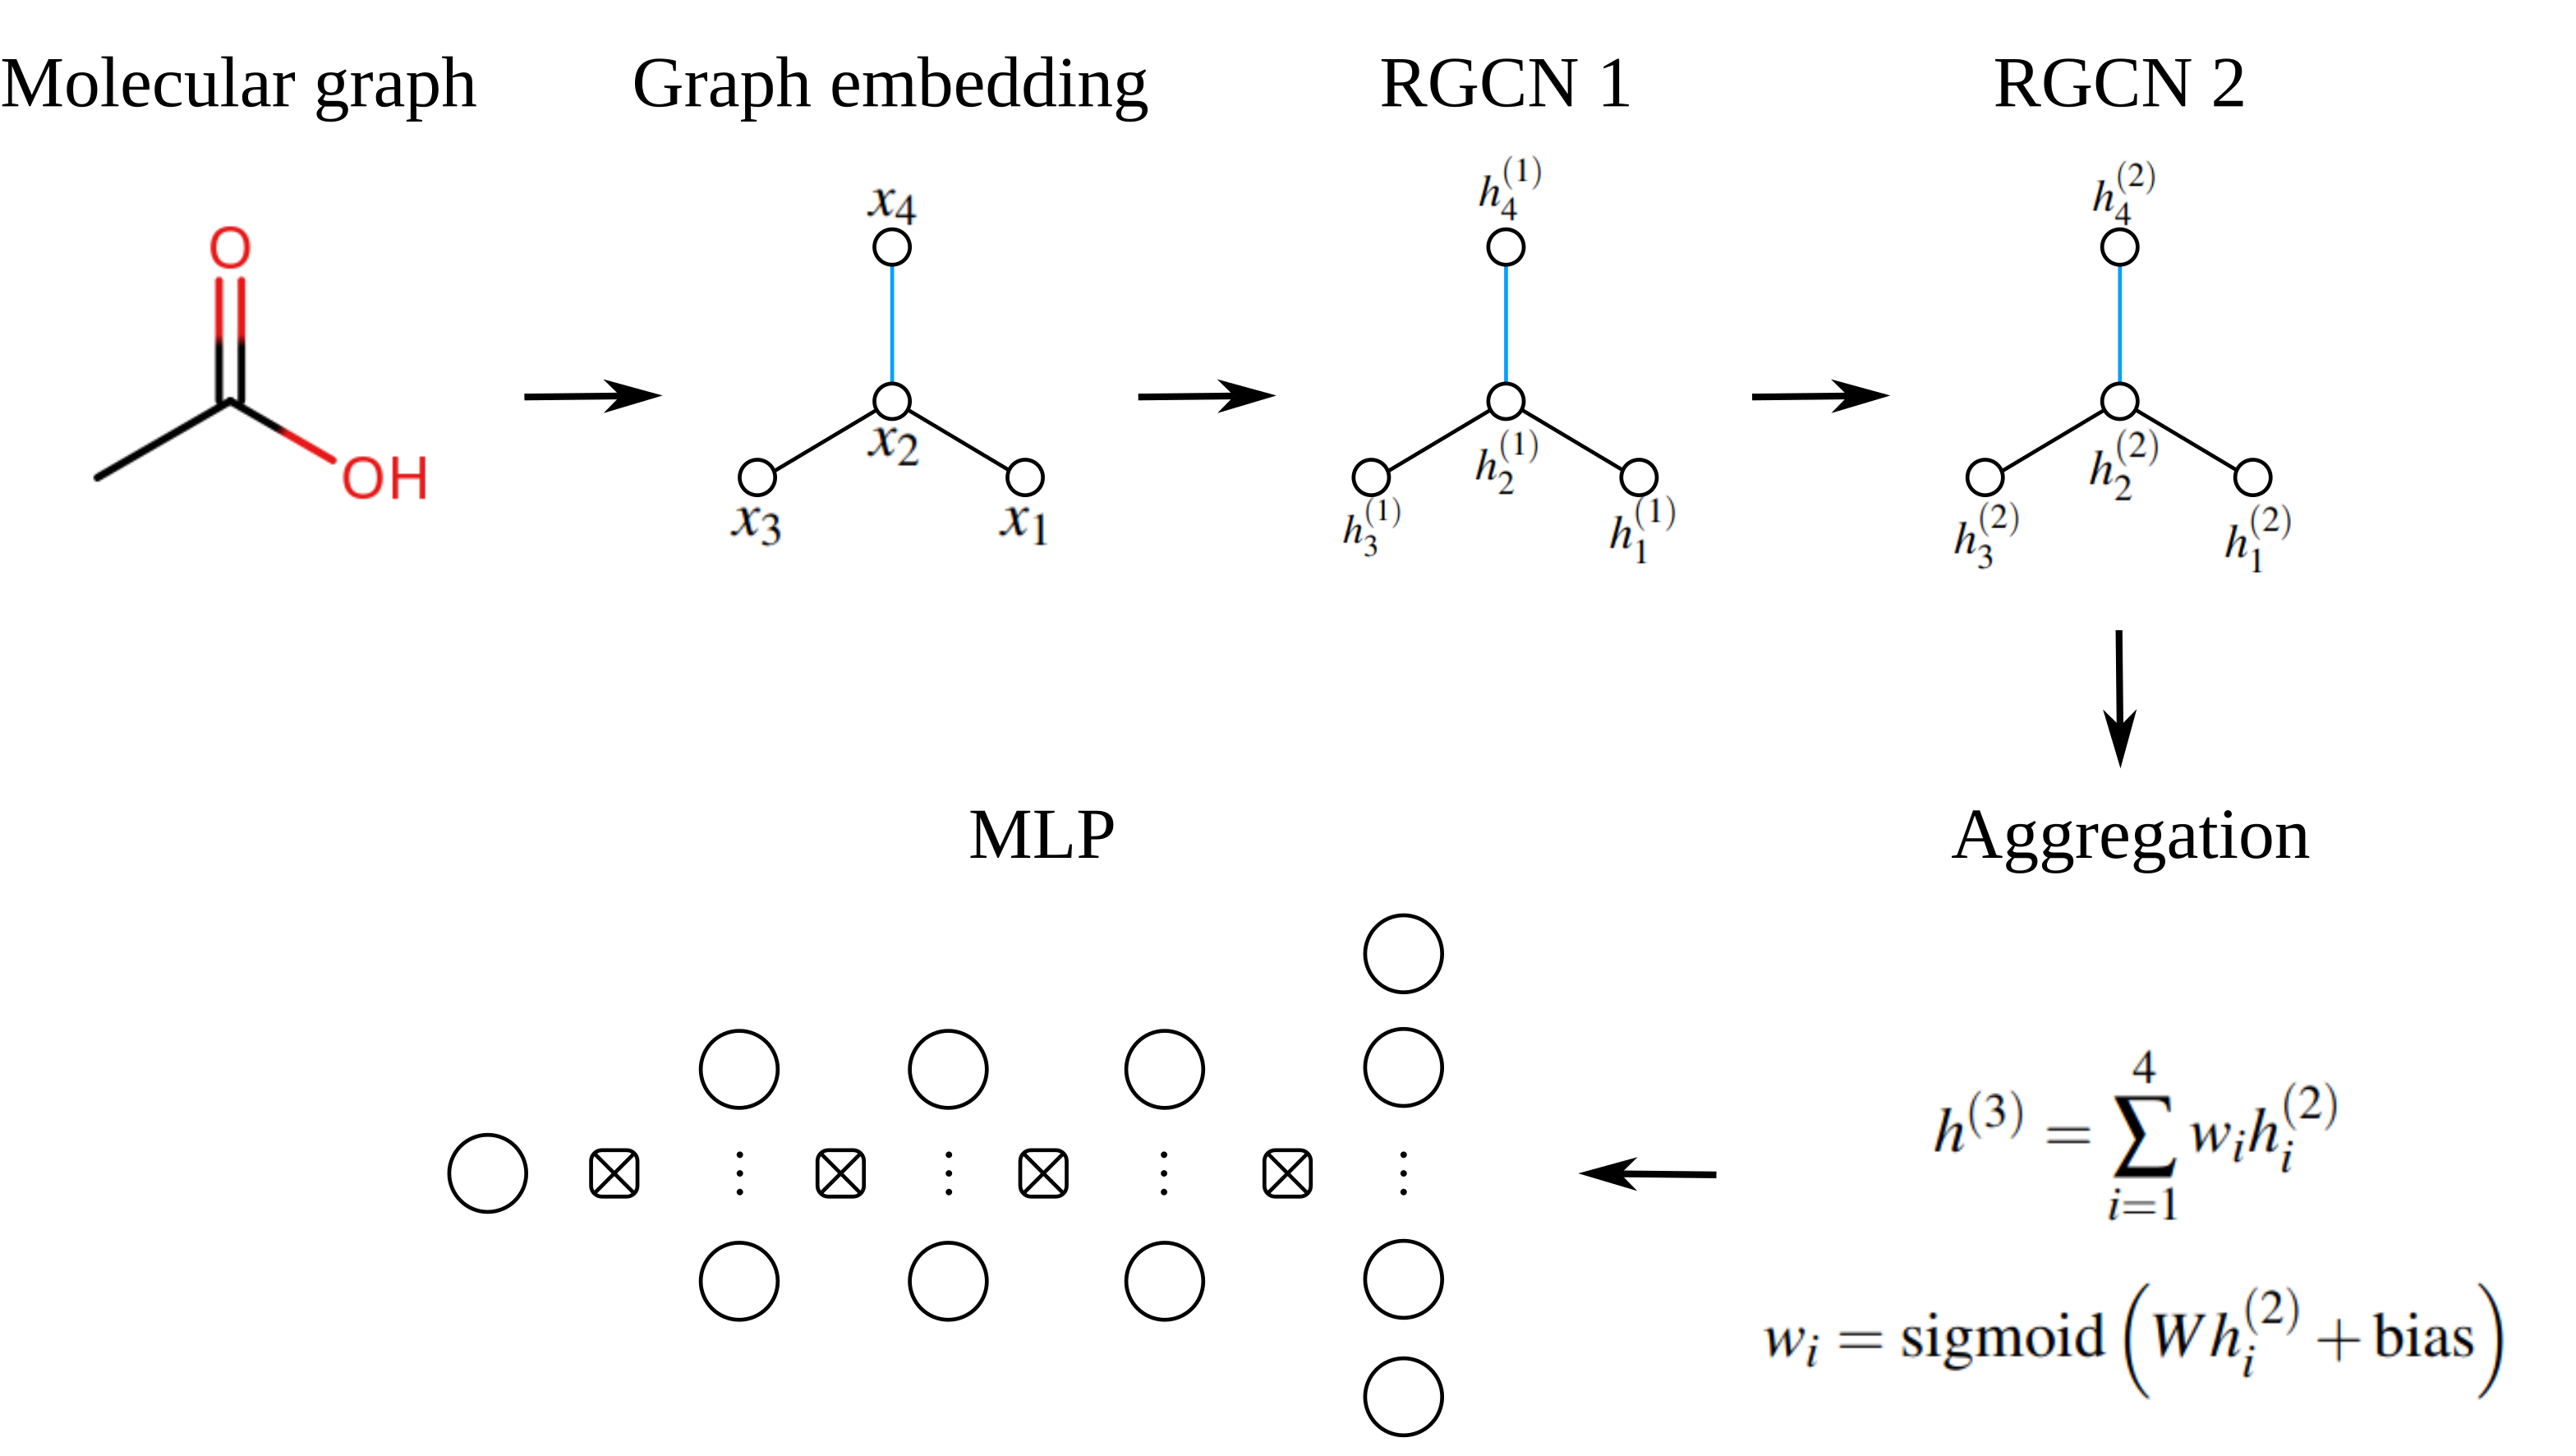
\includegraphics[scale=0.75]{../thesis/Fig/rgcn_model.png}
    \end{figure}
   
\end{frame}


\begin{frame}{Explanation pipeline}

    \begin{figure}[h]
        \centering
        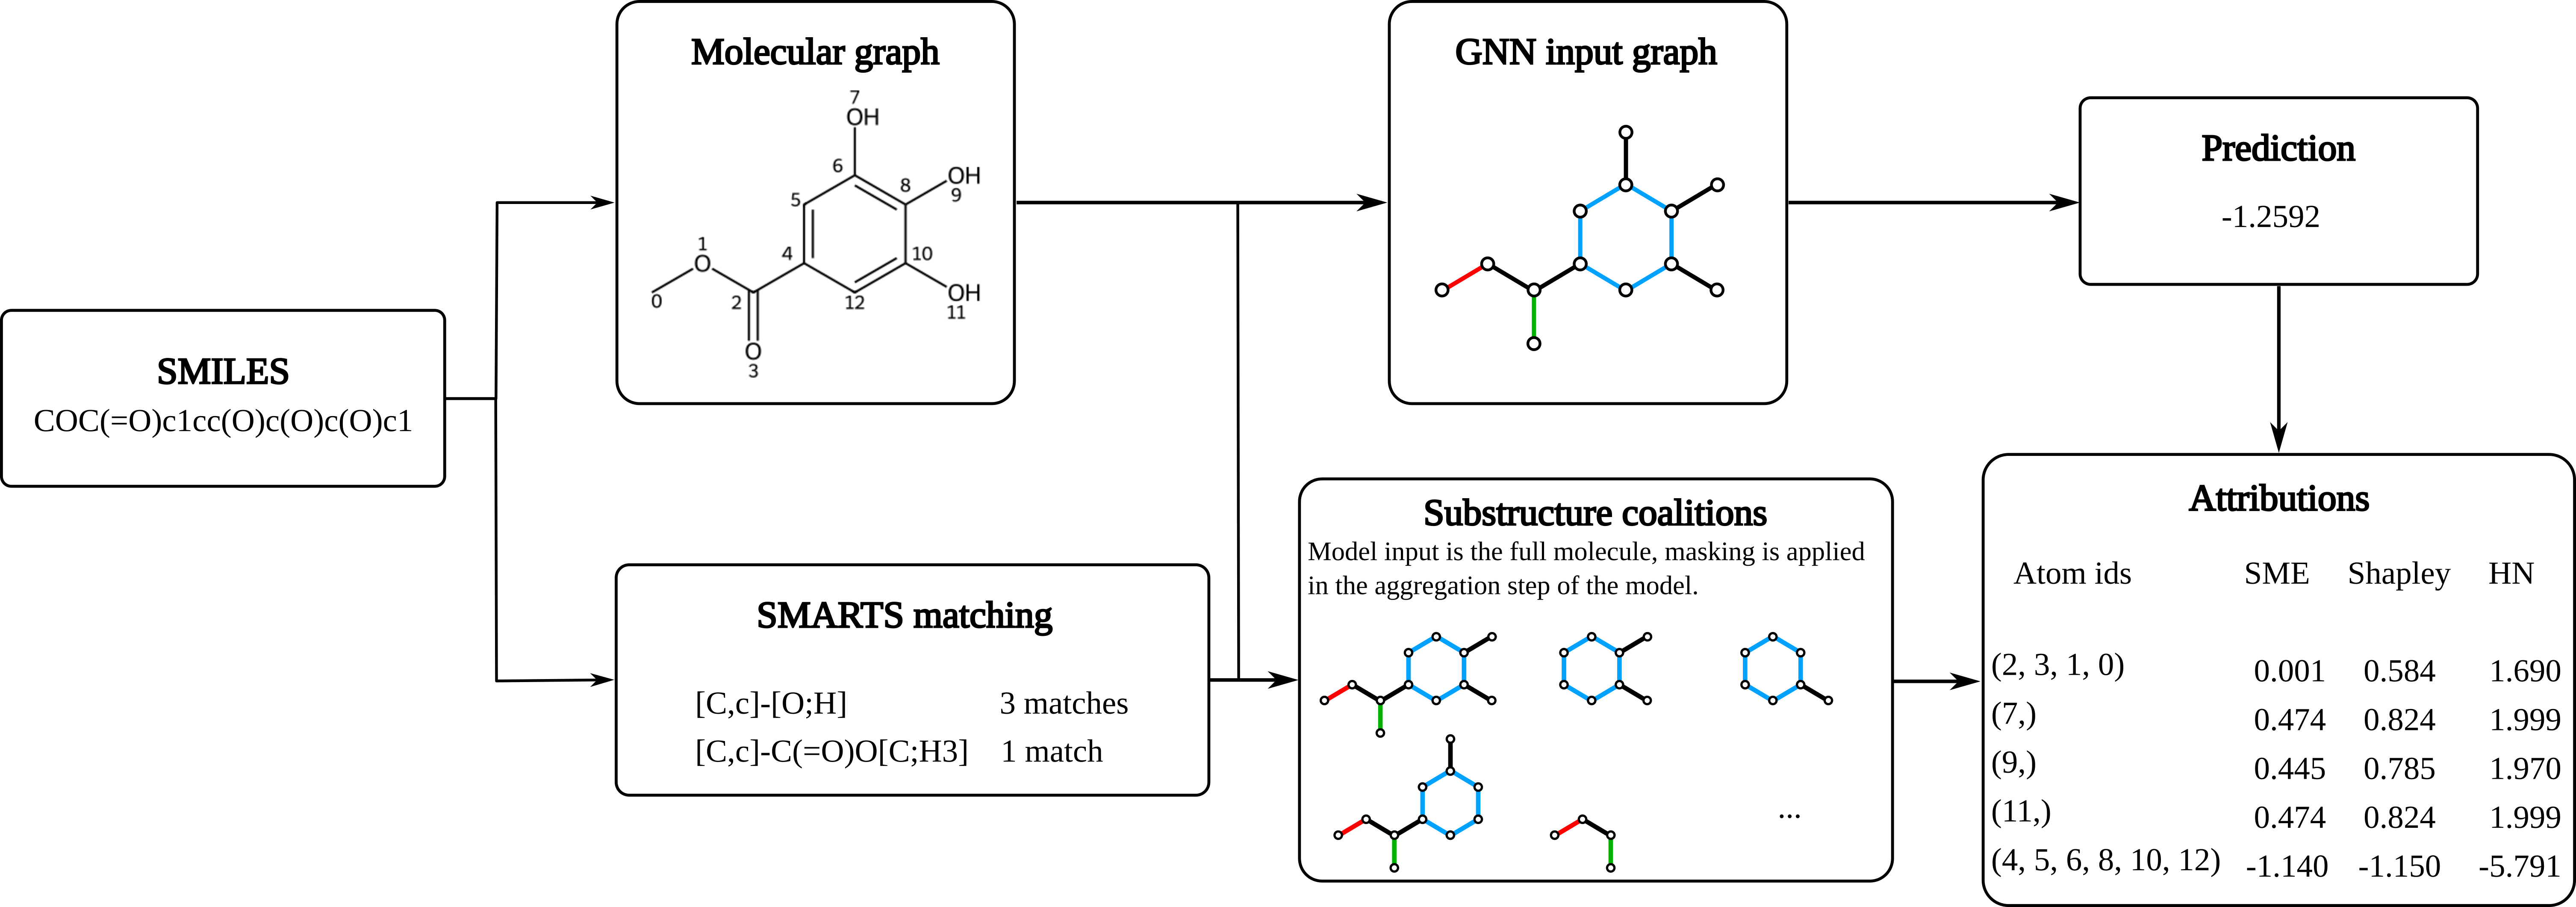
\includegraphics[scale=0.44]{./img/pipeline.png}
    \end{figure}

\end{frame}


\begin{frame}{RGCN is able to accurately predict expected water solubility}

    \begin{figure}[h]
        \centering
        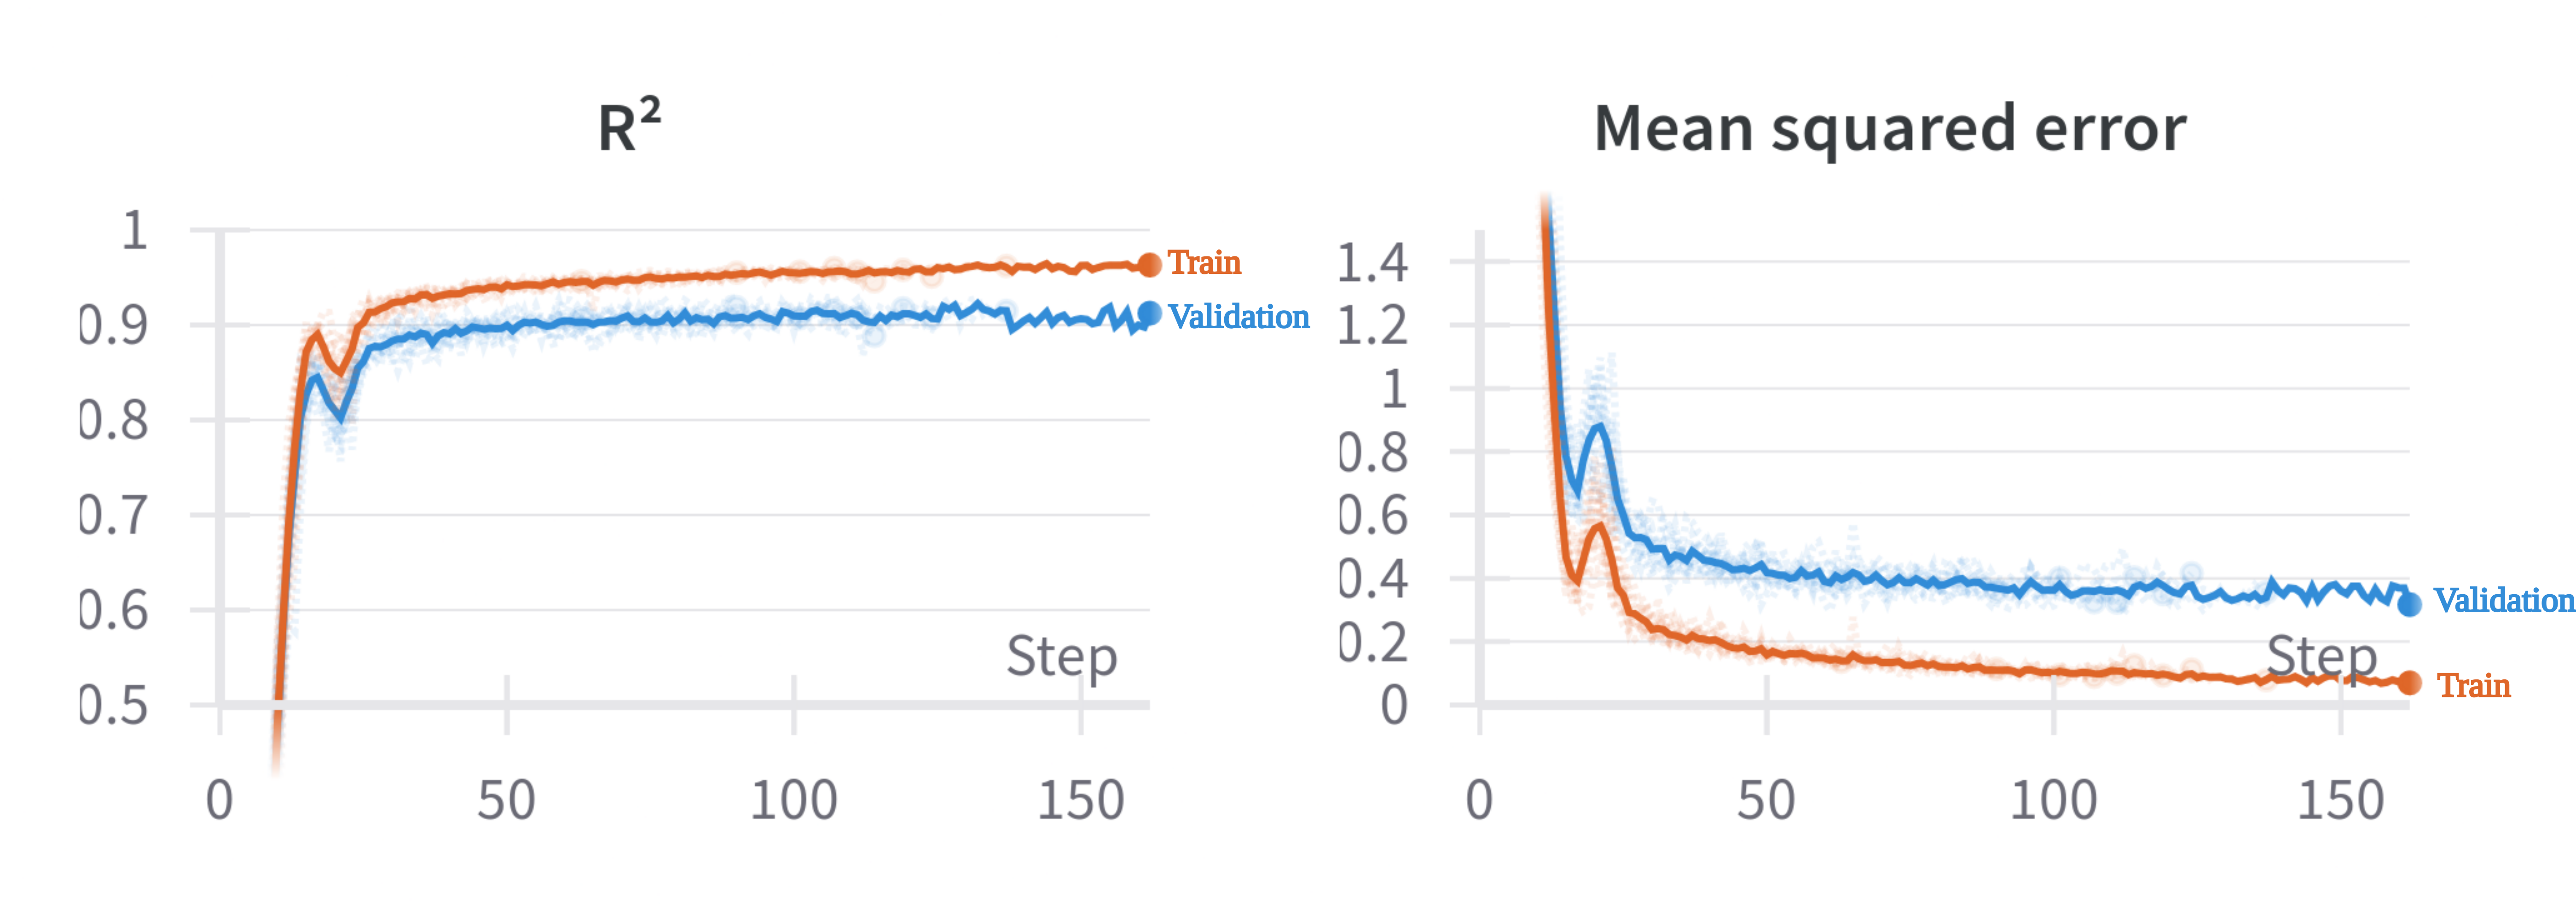
\includegraphics[scale=0.45]{./img/rgcn_performance.png}
    \end{figure}
   
\end{frame}


\begin{frame}{Different attribution methods can result in different explanations}

    \begin{figure}[h]
        \centering
        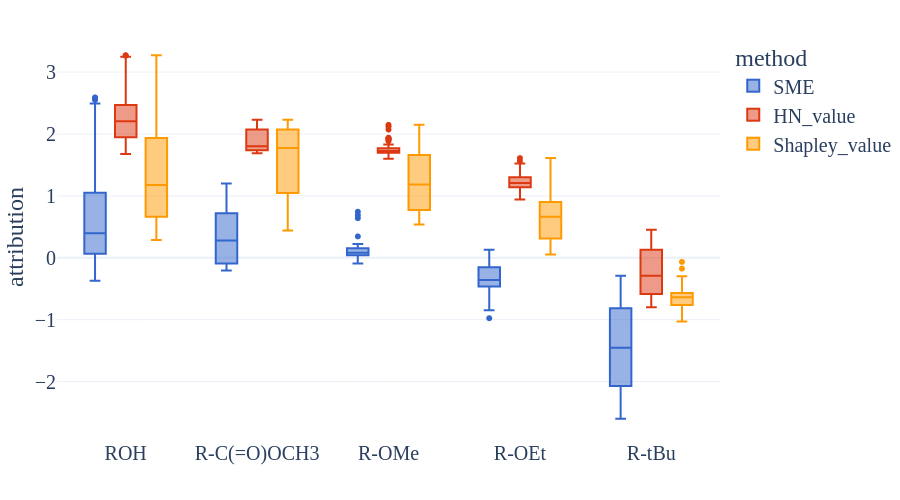
\includegraphics[scale=0.40]{../thesis/Fig/attribution_distribution_functional_groups.png}
    \end{figure}
  
\end{frame}


\begin{frame}{Different attribution methods can result in different explanations}

    \begin{figure}[h]
        \centering
        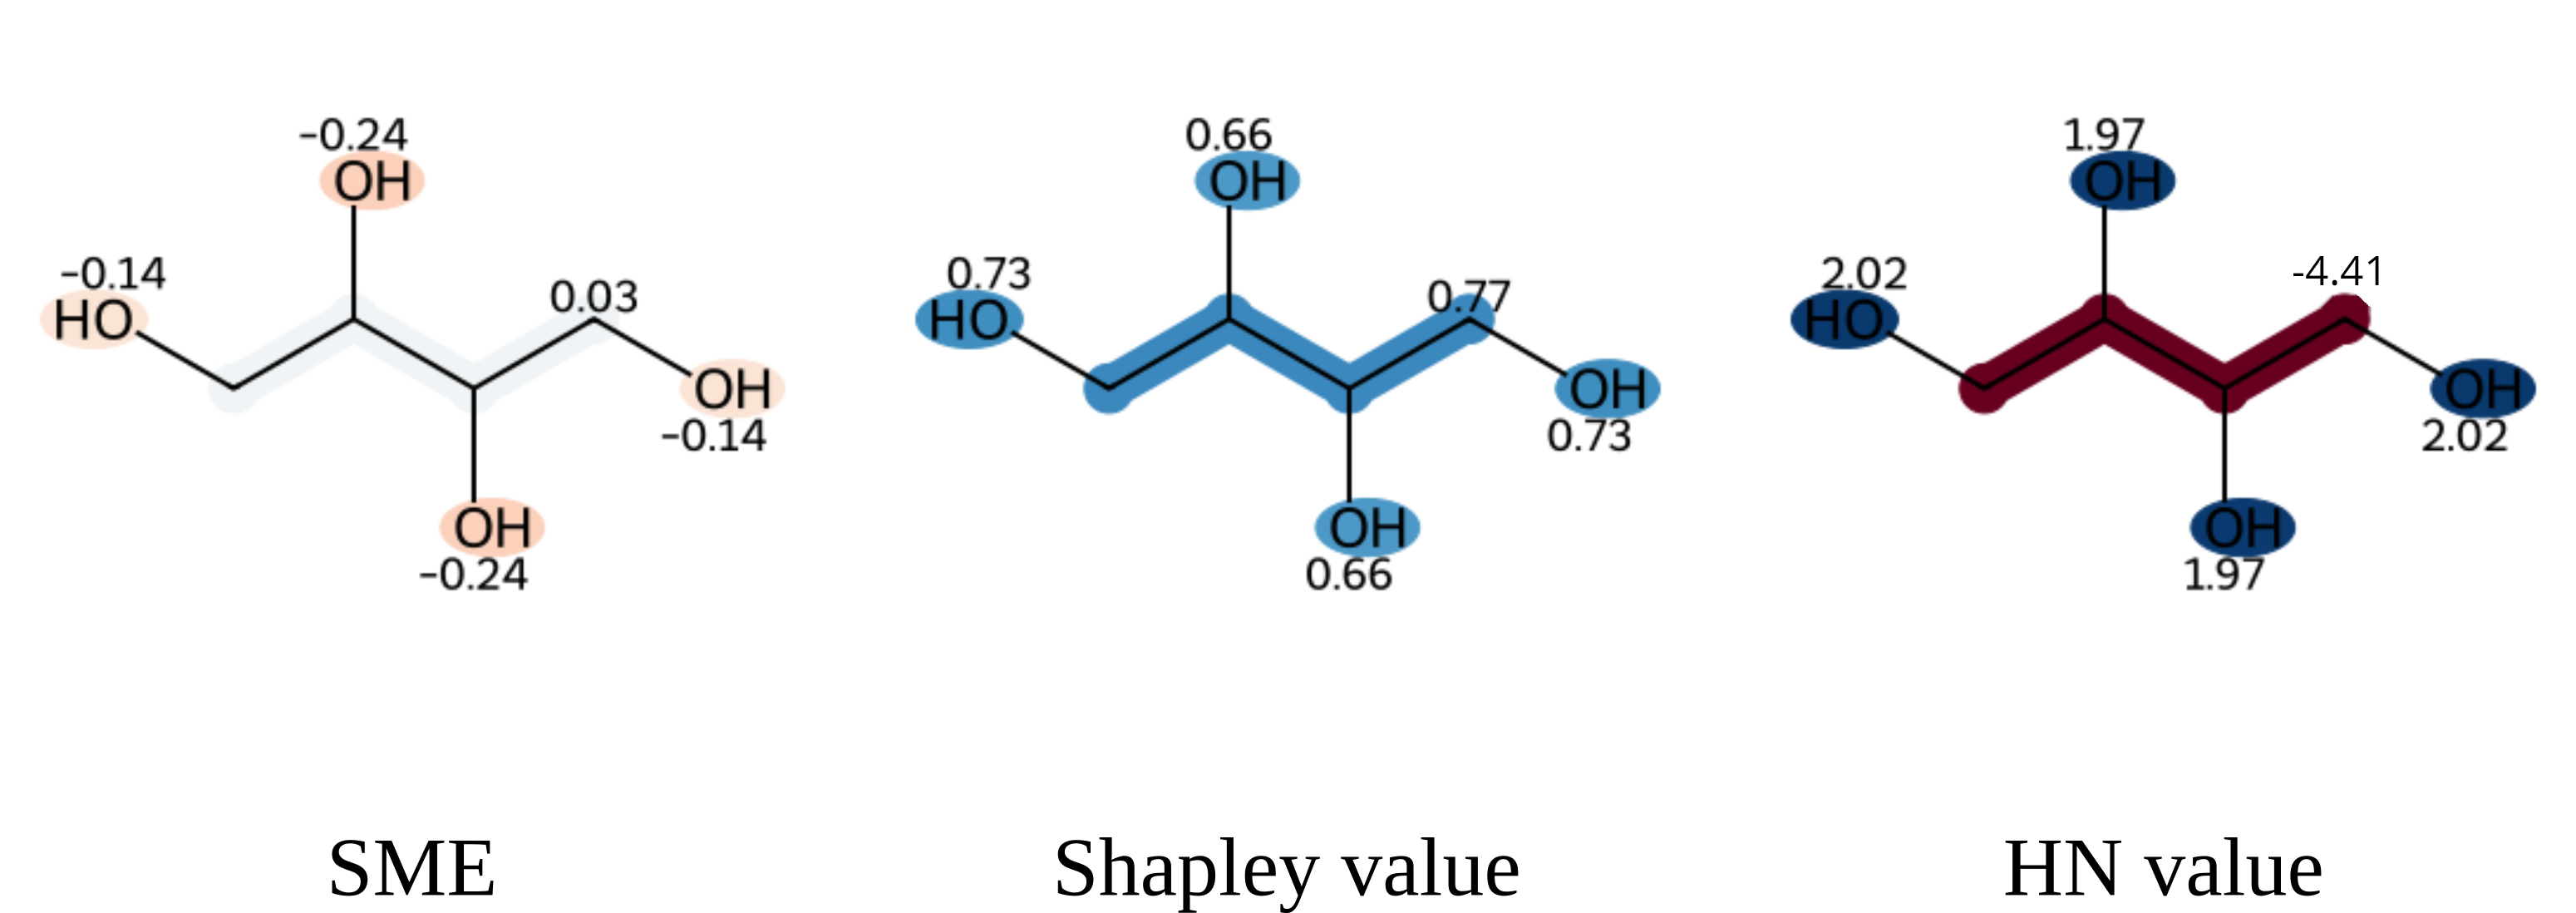
\includegraphics[scale=0.70]{../thesis/Fig/erythritol_explanations_2.png}
    \end{figure}
  
\end{frame}


\begin{frame}{Absolute prediction error is not associated with the Spearman rank correlation between different attribution methods}

    \begin{figure}[h]
        \centering
        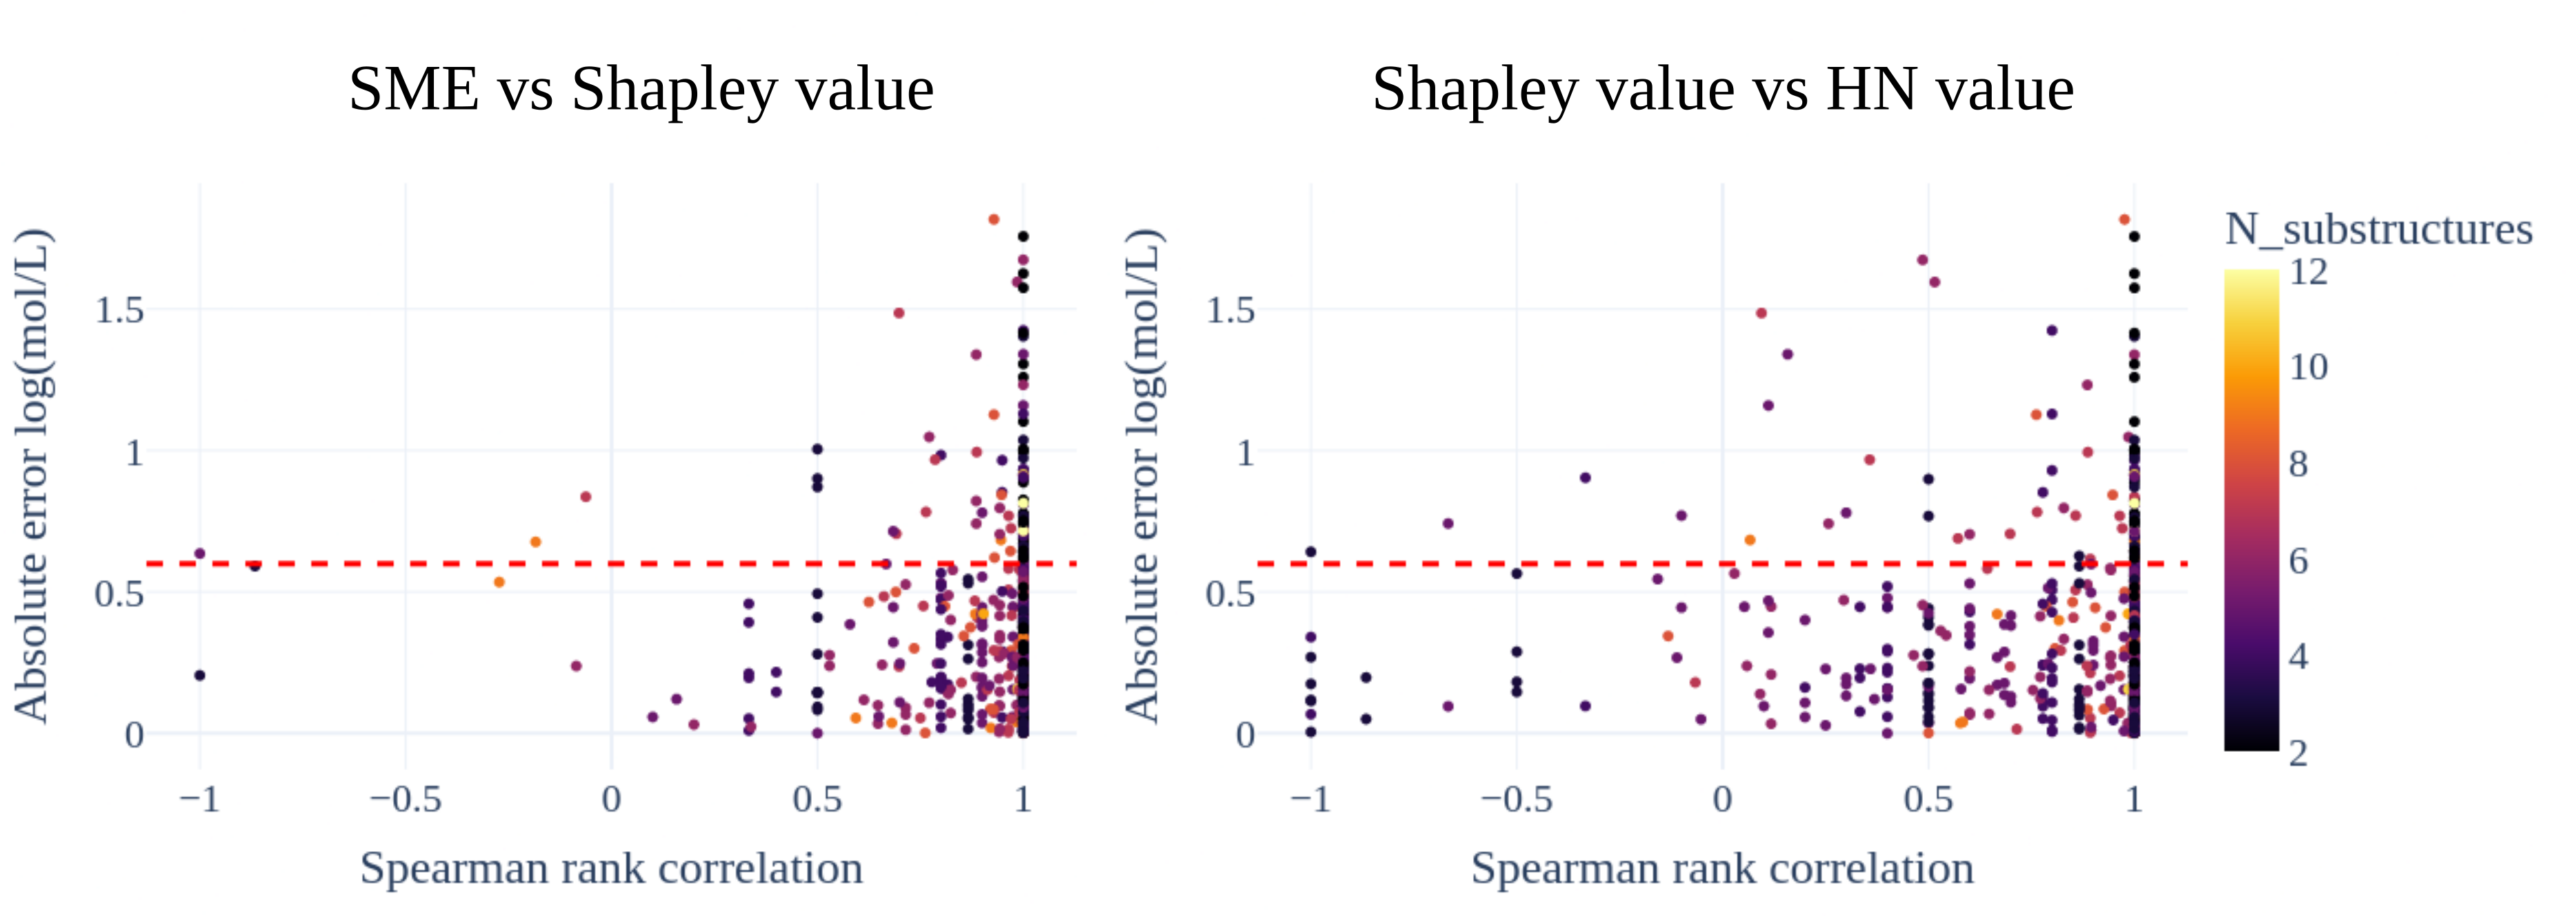
\includegraphics[scale=0.70]{../thesis/Fig/rmse_vs_rank_corr_attributions.png}
    \end{figure}
   
\end{frame}


\begin{frame}{All attribution methods have a similar ranking with chemical expectations}

    \begin{figure}[h]
        \centering
        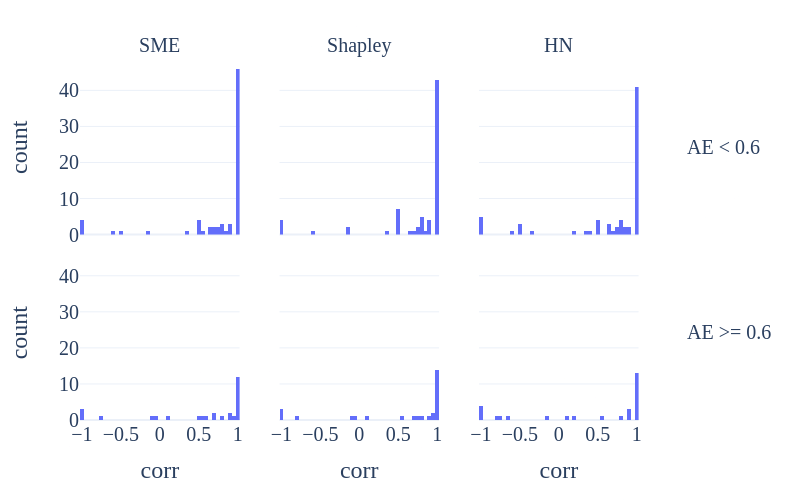
\includegraphics[scale=0.40]{../thesis/Fig/spearman_rank_correlation_manual_vs_attribution.png}
    \end{figure}
   
\end{frame}


\begin{frame}{All attribution methods have a similar ranking with chemical expectations}

    \begin{table}[h]
        \centering
        \caption{Average Spearman rank correlation between chemically ranked substructures and 
        a ranking based on attribution values.}
        \begin{tabular}{cccc}
        \toprule
        AE & SME & Shapley & HN \\
        \midrule
         < 0.6 & 0.7767 & 0.7708 & 0.6891 \\
        $\ge$ 0.6 & 0.5136 & 0.5482 & 0.3732 \\
         \bottomrule
        \end{tabular}
    \end{table}

    \begin{table}[h]
        \centering
        \caption{Friedman test results}
        \begin{tabular}{ccccc}
        \toprule
        AE & N & Statistic & df & p \\
        \midrule
         < 0.6 & 72 & 8.348 & 2 & 0.0154  \\
        $\ge$ 0.6 & 28 & 8.432 & 2 & 0.0148 \\
         \bottomrule
        \end{tabular}
    \end{table}

\end{frame}


\begin{frame}{All attribution methods are equally faithful to the ML model}

    \begin{figure}[h]
        \centering
        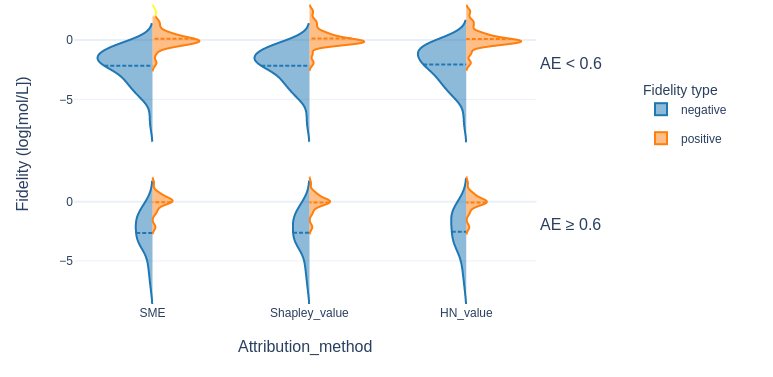
\includegraphics[scale=0.5]{../thesis/Fig/fidelity_2.png}
    \end{figure}
   
\end{frame}


\begin{frame}{All attribution methods are equally faithful to the ML model}

    \begin{figure}[h]
        \centering
        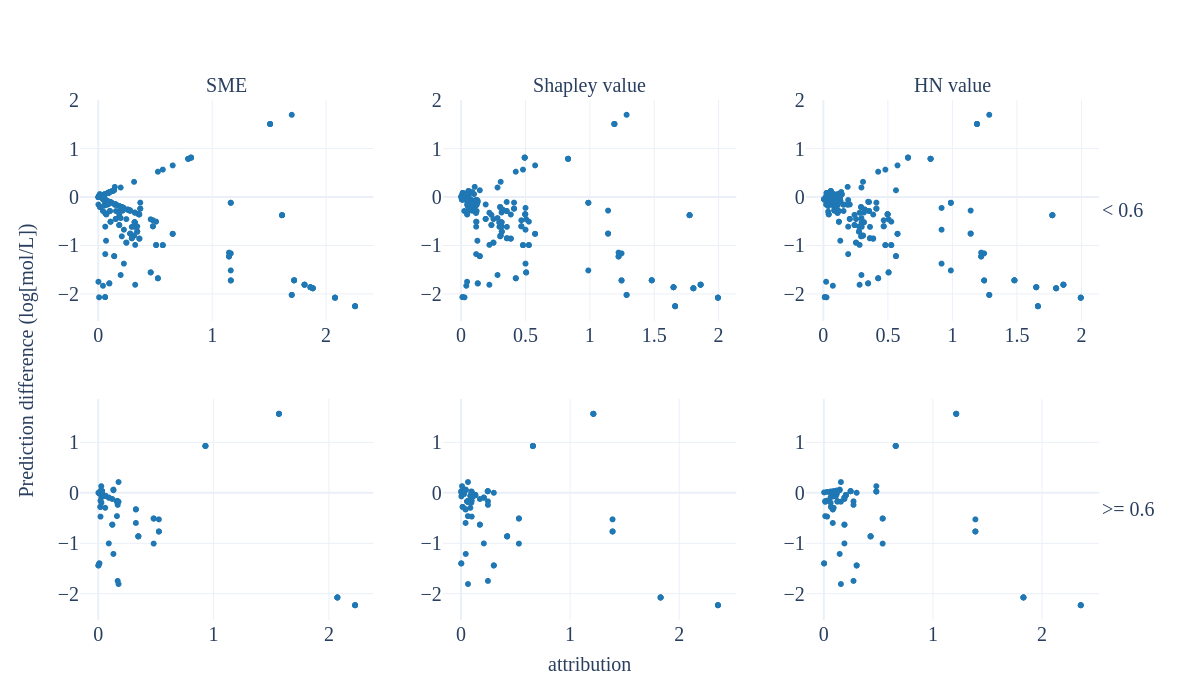
\includegraphics[scale=0.28]{../thesis/Fig/absolute_fidelity_3}
    \end{figure}
   
\end{frame}


\begin{frame}{Conclusions}

    \begin{itemize}
        \item HN attributions correctly capture the relative relation between functional groups
        \item All attribution methods result in similar ranking agreement with chemical expectations
        \item All attribution methods are equally faithful to the ML model
    \end{itemize}

    \begin{figure}[h]
        \centering
        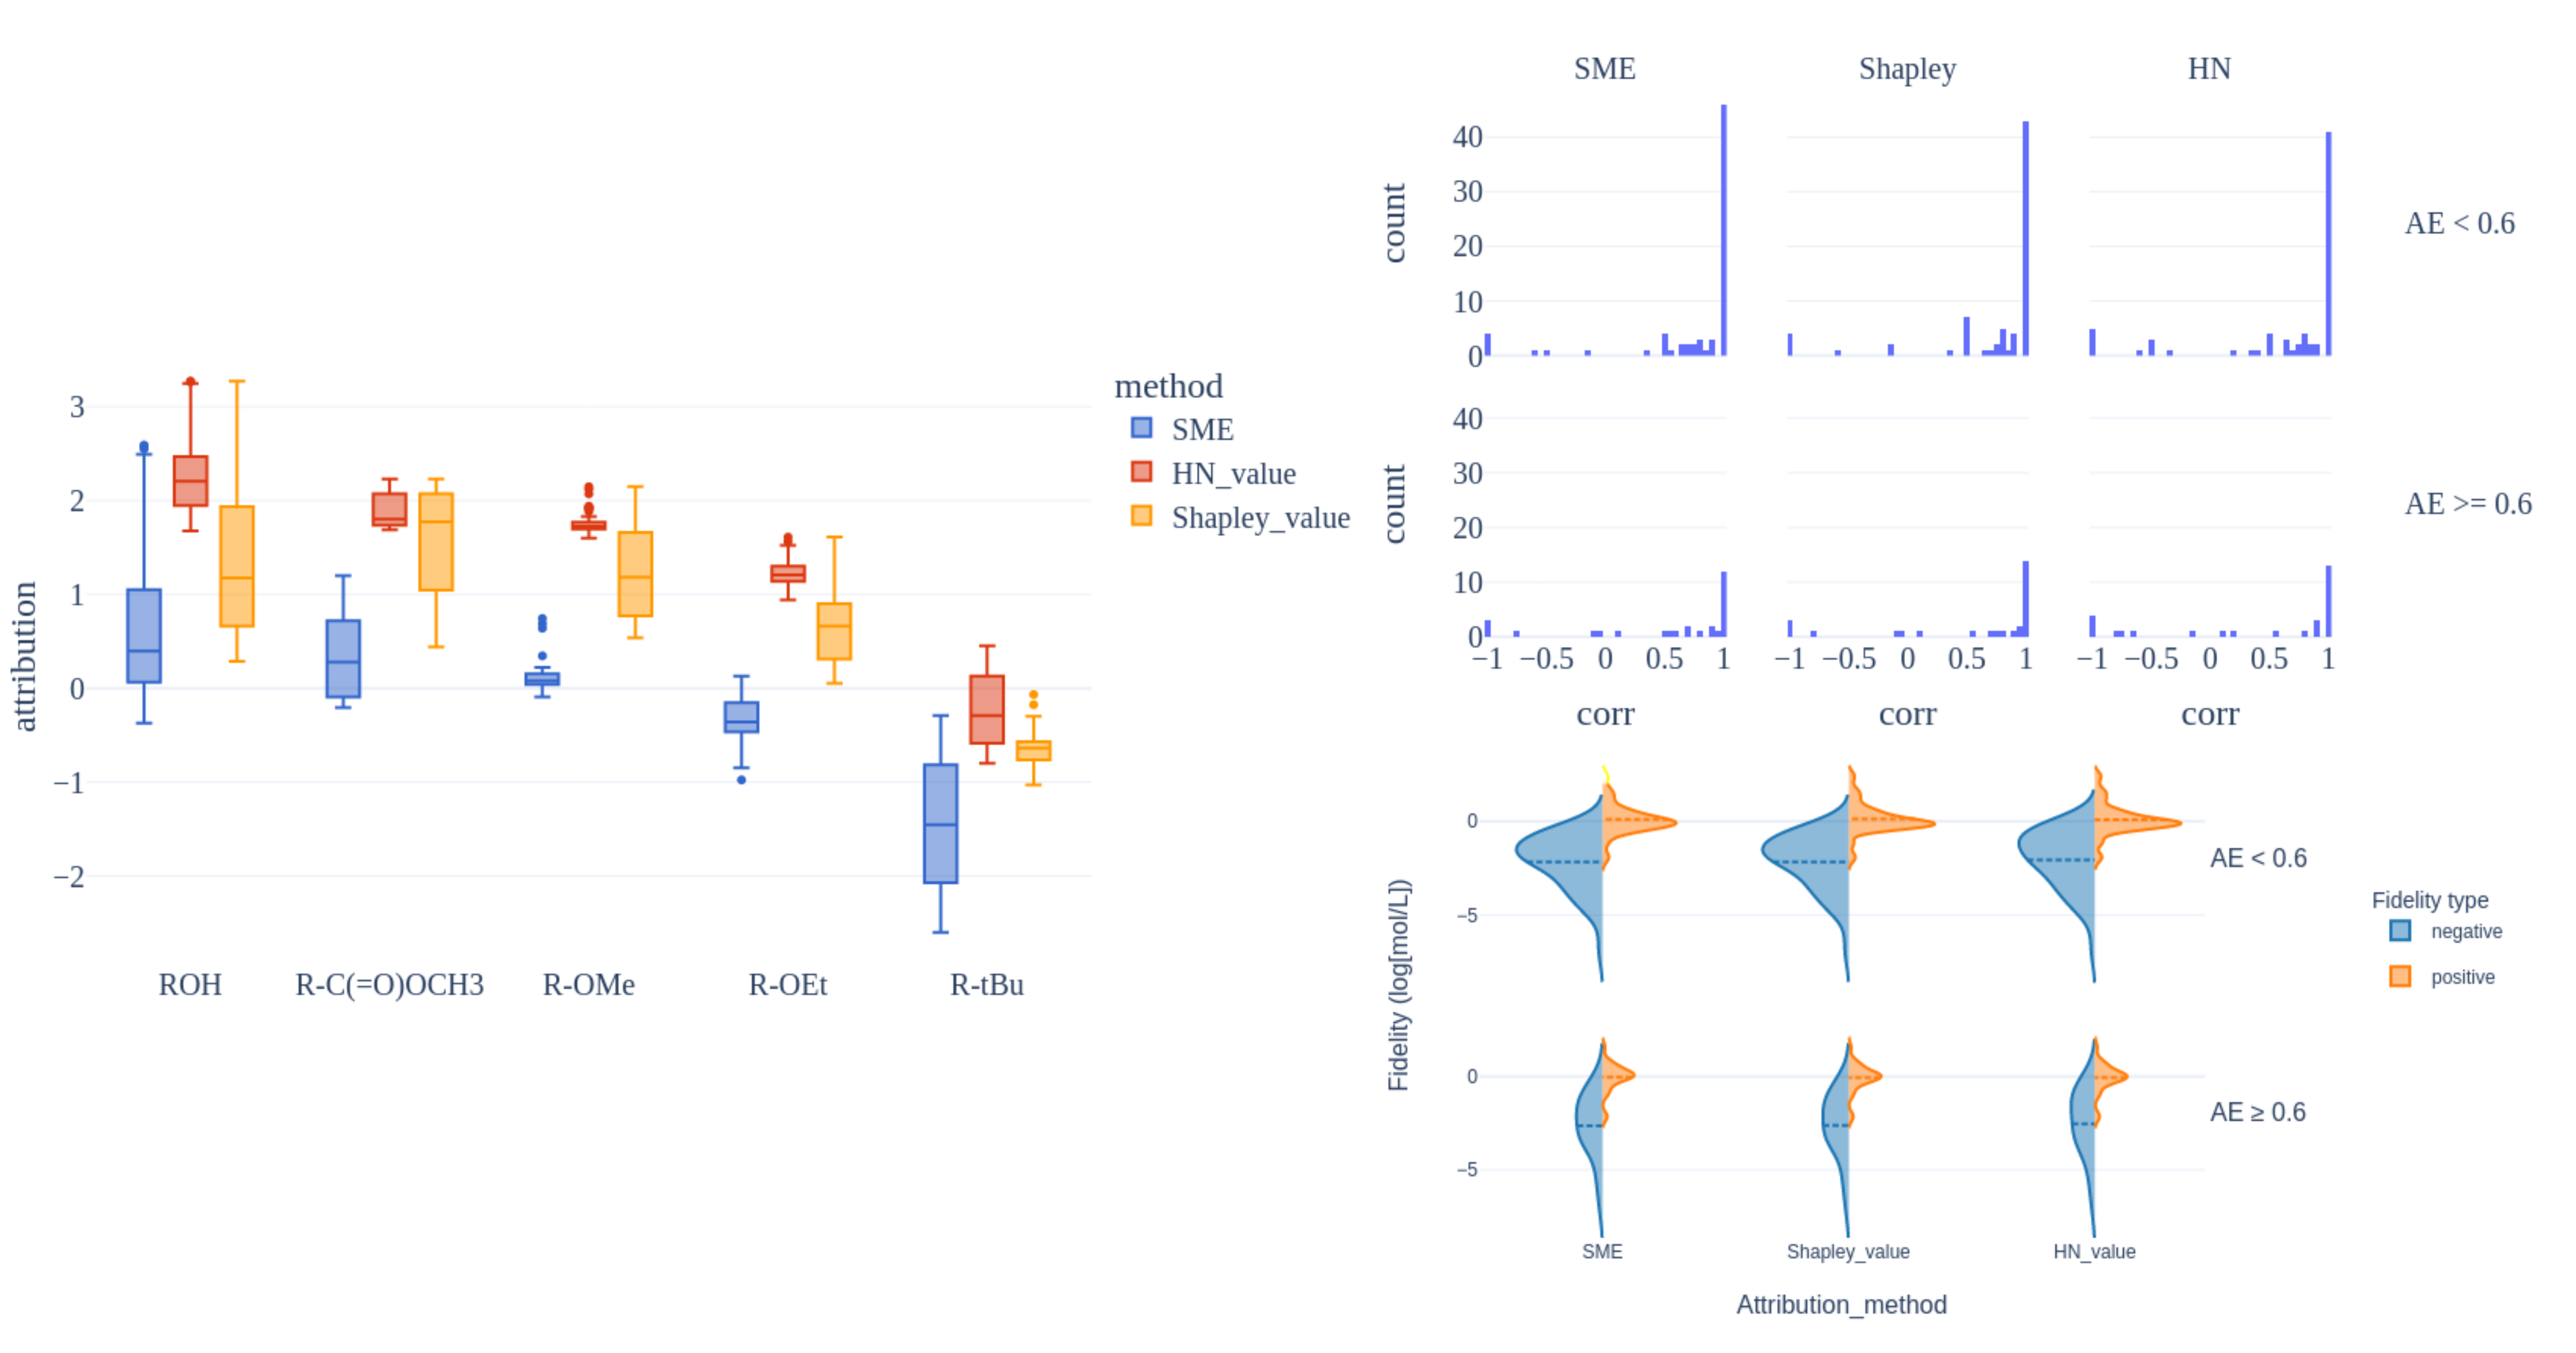
\includegraphics[scale=0.28]{./img/conclusion.png}
    \end{figure}

\end{frame}

\end{document}
